\noindent

\includegraphics[height=1.25cm]{images/pictograms/replication}

\includegraphics[height=1.25cm]{images/pictograms/benchmark}

\includegraphics[height=1.25cm]{images/pictograms/under_construction}

\includegraphics[height=1.25cm]{images/pictograms/FEM}

\includegraphics[height=1.25cm]{images/pictograms/paraview}

%%%%%%%%%%%%%%%%%%%%%%%%%%%%%%%%%%%%%%%%%%%%%%%%%%%%%%%%%%%%%%%%%%%%%%%%%%%%%%%%%%%%%%%%%%%%%%%%%%%

\begin{flushright} {\tiny {\color{gray} python\_codes/fieldstone\_126/text.tex}} \end{flushright}

%\lstinputlisting[language=bash,basicstyle=\small]{python_codes/template_keywords.key}

\par\noindent\rule{\textwidth}{0.4pt}

\begin{center}
\inpython
{\small Code: \url{https://github.com/cedrict/fieldstone/tree/master/python_codes/fieldstone_126}}
\end{center}

\par\noindent\rule{\textwidth}{0.4pt}

{\sl This stone was developed in collaboration with Donald Duck}. \index{contributors}{D. Duck}

\par\noindent\rule{\textwidth}{0.4pt}

Last revision: Jan. 23rd, 2025.

\par\noindent\rule{\textwidth}{0.4pt}

%%%%%%%%%%%%%%%%%%%%%%%%%%%%%%%%%%%%%%%%%%%%%%%%%%%%%%%%%%%%%%%%%%%%%%%%%%%%%%%%%%%%%%%%%%%%%%%%%%%


What follows is borrowed from paragraphs 43, 44 \& 45 of \textcite{grfr03} (2003).
Two main relations are used, expressing fluid mass conservation
\begin{equation}
\frac{\partial (\rho \upphi)}{\partial t} + \vec\nabla\cdot (\rho \vec{u}) = 0
\label{eq:por01}
\end{equation}
and Darcy's law\footnote{There is a minus sign in from of the permeability tensor missing at the 
beginning of paragraph 43}
\begin{equation}
\vec{u} = - {\bm K} \cdot (\vec{\nabla} P + \rho \vec{g})
\label{eq:por00}
\end{equation}
where $\rho$ is the density of the fluid, $\upphi$ is the
connected mean porosity of the rock, $\vec{u}$ is the Darcy flow
rate\footnote{The authors state that it is ``fluid particle velocity times porosity''. 
I don't get it}, ${\bm K}$ is the permeability tensor, $P$ is the total pore pressure and $\vec{g}$ is
the gravity. 

\underline{Remark:} 
At this stage one must realize that the standard Darcy flow law is $\vec{u} = - {\bm K}/\eta_f \cdot (\vec{\nabla} P - \rho_f \vec{g})$. In this case I don't know why the viscosity has disappeared. The permeability\footnote{\url{https://en.wikipedia.org/wiki/Permeability_(materials_science)}} $K$ should be in $\si{\square\meter}$ but here it would then be in $\si{\square\meter\per\pascal\per\second}$. Also the minus sign is probably linked to the fact that the vertical axis is pointing down instead of up. 



First, during the evolution, we consider that the density 
$\rho = \rho' + \rho_m$ will evolve in time of an amount $\rho'$ 
around its local mean value $\rho_m$ ,

Then Eq.~\eqref{eq:por01} becomes,
\begin{eqnarray}
\frac{\partial ((\rho'+\rho_m) \upphi)}{\partial t} + \vec\nabla\cdot ((\rho'+\rho_m) \vec{u}) &=& 0 
\nn\\
(\rho'+\rho_m) \frac{\partial \upphi}{\partial t} 
+\upphi \frac{\partial (\rho'+\rho_m)}{\partial t} 
+ \vec\nabla\cdot ((\rho'+\rho_m) \vec{u}) &=& 0
\nn\\
(\rho' + \rho_m) \frac{\partial \upphi}{\partial t} 
+\upphi \frac{\partial \rho'}{\partial t} 
+\upphi \frac{\partial \rho_m}{\partial t} 
+ \vec\nabla\cdot ((\rho'+\rho_m) \vec{u}) 
&=& 0 \nn
\end{eqnarray}
Since $\rho_m$ is taken to be constant and homogeneous in the crust
then $\partial_t \rho_m =0$ %and $\vec\nabla \rho_m=\vec{0}$
and neglecting the terms $\rho'$ compared to $\rho_m$ we can write
\begin{equation}
(\underbrace{\rho' }_{neglect} + \rho_m )\frac{\partial \upphi}{\partial t} 
+\upphi \frac{\partial \rho'}{\partial t} 
+\upphi \underbrace{\frac{\partial \rho_m}{\partial t} }_{=0}
+ \vec\nabla\cdot ((\underbrace{\rho'}_{neglect}+\rho_m) \vec{u}) = 0
\end{equation}
and finally obtain:
\begin{equation}
\boxed{
\rho_m \frac{\partial \upphi}{\partial t} 
+\upphi \frac{\partial \rho' }{\partial t} 
+ \vec\nabla\cdot (\rho_m \vec{u}) = 0
}
\label{eq:por10}
\end{equation}
which is Eq.~(9) in the paper.

Second, we consider that the total pore pressure $P$ can
be decomposed as $P = p + P_{hydro}$ such that $P_{hydro}$ is the
hydrostatic pressure verifying $\vec\nabla P_{hydro} + \rho_m \vec{g} = \vec{0}$. 
Then Eq.~\eqref{eq:por00} becomes
\begin{align}
\vec{u} &= -{\bm K} \cdot (\vec{\nabla} (p + P_{hydro}) + (\rho'+\rho_m) \vec{g}) 
\end{align}
Again, neglecting $\rho'$ compared to $\rho_m$, we arrive at
\begin{equation}
\boxed{
\vec{u} = -{\bm K} \cdot \vec{\nabla} p  
}
\label{eq:por21}
\end{equation}

Also in the paper the authors consider that the principal directions of the permeability
tensor ${\bm K}$ are the axes of the fault frame $x,z$, which means
that the anisotropy of the permeability takes the natural
direction of the fault. This last assumption seems reasonable
if the fault has a constant straight and vertical shape.
This means that ${\bm K}$ is diagonal:
\begin{equation}
{\bm K}(x,z,t) = \left(\begin{array}{cc}
K_x(x,z,t) & 0 \\ 
0 & K_z(x,z,t)
\end{array}\right)
\label{eq:por22}
\end{equation}
so that indeed
\begin{equation}
u_x = -K_x \partial_x p
\qquad
\text{and}
\qquad
u_y = -K_y \partial_y p
\label{eq:por11}
\end{equation}
which is Eq.~(10) of the paper.
The two permeabilities $K_z$ and $K_x$ are chosen to express a high anisotropy with a ratio 
$K_z/K_x =100$. This ratio is chosen to allow a reasonable fluid transfer across the fault zone.

It is assumed that the variation of the density of the fluid $\rho'$ 
is only due to the variation of the fluid pressure $p$. This dependence is simply
expressed with a compressibility factor $C_f = \frac{1}{\rho_m}\frac{\partial \rho'}{\partial p} $
taken as a constant. $C_f$ is expressed in $\si{\per\pascal}$.

We can write this equation as follows:
\begin{equation}
C_f = \frac{1}{\rho_m}\frac{\partial \rho'}{\partial p} = 
\frac{1}{\rho_m}\frac{\partial \rho'}{\partial t}\frac{\partial t}{\partial p}
\qquad
\text{or,}
\qquad
\frac{\partial \rho'}{\partial t} = \rho_m C_f  \frac{\partial p}{\partial t}
\label{eq:por20}
\end{equation}
which is the equation at the bottom of page 15 of the paper.

It is also assumed that the porosity is such that $\upphi=\upphi_m + \upphi'$
and that it will vary at two independent
amplitude scales. The $\upphi_m$ is the mean local porosity that
varies strongly and heterogeneously in time because of the
kinetics of the crack sealing process (see below). The $\upphi'$ is
the smaller variation of the porosity due to the fluid pressure variation.

Therefore we write
\begin{equation}
\frac{\partial \upphi}{\partial t}
=\frac{\partial \upphi_m}{\partial t} +\frac{\partial \upphi'}{\partial t}
=\frac{\partial \upphi_m}{\partial t} +\frac{\partial \upphi'}{\partial p} \frac{\partial p}{\partial t}
\label{eq:por25}
\end{equation}
The pore pressure dependence of $\upphi'$ is defined by a
simple matrix compressibility factor
\begin{equation}
C_m = \frac{1}{\upphi_m}\frac{\partial \upphi'}{\partial p}
\label{eq:por24}
\end{equation}
Its units are also \si{\per\pascal}.
Rigorously, by following the Biot theory of poroelasticity,
reformulated later by [Rice and Cleary, 1976], the pore
pressure should also depend on the variations of the state of
total stress or the state of strain of the crust. For simplicity,
we will consider that the state of total stress of the crust will
not change significantly during the pressurization. This
rough approximation is the main limit of the model. Indeed
it does not consider the interaction involved by the
poroelastic theory, which is out of the scope of this paper.
Therefore, by considering, in first approximation, that the
variations of the state of total stress of the crust are small,
we have 
\begin{equation}
C_m = C_d \left[ \frac{C_d - C_s}{\upphi_m C_s } - 1  \right],
\end{equation}
where $C_s$ is the compressibility of the pure solid part and $C_d$ is the
compressibility of the skeleton, i.e., the dried solid part
containing the pores. During the simulation, the mean
porosity $\upphi_m$ will decrease significantly in time, due to the
pressure solution, but at the same time $C_d$ tends to reach $C_s$.
This is why we assume that the compressibility of the
matrix $C_m$ can reasonably be taken as a constant. 

Having stated all this it is now time to put it all together.
We start by combining equations \eqref{eq:por10} and \eqref{eq:por11}:

\begin{eqnarray}
\rho_m \frac{\partial \upphi}{\partial t} 
+\upphi \frac{\partial \rho' }{\partial t} 
+ \vec\nabla\cdot (\rho_m \vec{u}) &=& 0 \nn
\end{eqnarray}
Now using Eqs.~\eqref{eq:por21} and \eqref{eq:por20} leads to
\begin{eqnarray}
\rho_m \frac{\partial \upphi}{\partial t} 
+\upphi \rho_m C_f \frac{\partial p}{\partial t} 
+ \vec\nabla\cdot (- \rho_m {\bm K} \cdot \vec\nabla p) &=& 0 
\end{eqnarray}
Since $\rho_m$ is constant it can be taken out of the divergence term 
and eliminated from the equations:
\begin{eqnarray}
 \frac{\partial \upphi}{\partial t} 
+\upphi  C_f \frac{\partial p}{\partial t} 
+ \vec\nabla\cdot (- {\bm K} \cdot \vec\nabla p) &=& 0 
\end{eqnarray}
Using Eq.~\eqref{eq:por22} we can write:
\begin{eqnarray}
\frac{\partial \upphi}{\partial t} 
+\upphi  C_f \frac{\partial p}{\partial t} 
- \frac{\partial}{\partial x} \left( K_x \frac{\partial p}{\partial x} \right) 
- \frac{\partial}{\partial z} \left( K_z \frac{\partial p}{\partial z} \right) 
&=& 0 
\end{eqnarray}
Combining Eq.~\eqref{eq:por25} and \eqref{eq:por24} we can write
\[
\frac{\partial \upphi}{\partial t}
=\frac{\partial \upphi_m}{\partial t} +\frac{\partial \upphi'}{\partial p} \frac{\partial p}{\partial t}
=\frac{\partial \upphi_m}{\partial t} + C_m \upphi_m \frac{\partial p}{\partial t}
\]
which we insert in the equation above to obtain
\begin{eqnarray}
\frac{\partial \upphi_m}{\partial t} + C_m \upphi_m \frac{\partial p}{\partial t}
+\upphi  C_f \frac{\partial p}{\partial t} 
- \frac{\partial}{\partial x} \left( K_x \frac{\partial p}{\partial x} \right) 
- \frac{\partial}{\partial z} \left( K_z \frac{\partial p}{\partial z} \right) 
&=& 0 \nn\\
%\frac{\partial \upphi_m}{\partial t} 
%+ (C_m \upphi_m 
%+ \upphi  C_f )\frac{\partial p}{\partial t} 
%- \frac{\partial}{\partial x} \left( K_x \frac{\partial p}{\partial x} \right) 
%- \frac{\partial}{\partial z} \left( K_z \frac{\partial p}{\partial z} \right) 
%&=& 0 \nn\\
\frac{\partial \upphi_m}{\partial t} 
+ (C_m \upphi_m 
+ (\upphi_m+\upphi' ) C_f )\frac{\partial p}{\partial t} 
- \frac{\partial}{\partial x} \left( K_x \frac{\partial p}{\partial x} \right) 
- \frac{\partial}{\partial z} \left( K_z \frac{\partial p}{\partial z} \right) 
&=& 0 
\end{eqnarray}
Neglecting $\upphi'$ in the lhs yields
\begin{eqnarray}
\frac{\partial \upphi_m}{\partial t} 
+ (C_m \upphi_m 
+ \upphi_m C_f )\frac{\partial p}{\partial t} 
- \frac{\partial}{\partial x} \left( K_x \frac{\partial p}{\partial x} \right) 
- \frac{\partial}{\partial z} \left( K_z \frac{\partial p}{\partial z} \right) 
&=& 0 
\end{eqnarray}
or, defining $C=C_f+C_m$:
\begin{equation}
\boxed{
\frac{\partial \upphi_m}{\partial t} 
+ C \upphi_m \frac{\partial p}{\partial t} 
=\frac{\partial}{\partial x} \left( K_x \frac{\partial p}{\partial x} \right) 
+ \frac{\partial}{\partial z} \left( K_z \frac{\partial p}{\partial z} \right)
}
\label{eq:por02}
\end{equation}
which is Eq.~(11) of the paper, albeit in spirit only\footnote{I believe that the equation in the 
paper is wrong: the term $(\partial_x+\partial_z)$ makes no sense.
Also the authors state that in order to arrive at this equation 
``we neglect the remaining second
order terms involving the product $\upphi'\rho'$''
which I do not understand since $\rho'$ does not appear anywhere...}.

$C$ expresses the mean matrix-fluid compressibility and $\upphi_m C$ represents the 
pressure storativity\footnote{\url{https://en.wikipedia.org/wiki/Specific_storage}}. 
This storativity will naturally decrease with
the porosity $\upphi_m$ because of the crack sealing process.
The expression \eqref{eq:por02} is a linear diffusion equation
with time and space dependent coefficients and a forcing
term $\partial \upphi_m/\partial t$. The porosity $\upphi$ is expressed as a function of
space and time following natural observations (Figure 9c,
t = 0) and crack sealing modeling (Figures 8b and 8c),
respectively:
\begin{equation}
\upphi_m(x,z,t)=\upphi_0 \exp (-x/L) \exp (-t/\tau(z))
\label{eq:por03}
\end{equation}
and, consequently,
\begin{equation}
\frac{\partial \upphi_m}{\partial t} = -\frac{\upphi_0}{\tau(z)} \exp (-x/L) \exp (-t/\tau(z)) 
\label{eq:por04}
\end{equation}
$L$ is the characteristic distance for the exponential decrease
of the porosity after each earthquake (distance for which the
maximum porosity $\upphi_0$ along the fault is divided by $e$).
The $\tau(z)$ is the characteristic time of the sealing process
(time during which the porosity is divided by $e$). The
shape of $\tau(z)$ as been derived from a stratified crust with
different rates of compaction using the results of the crack
sealing modeling (see Fig.~9a). In the upper crust, we
assume the predominance of the calcite rate of crack sealing
at low temperature and pressure while in the deeper crust we
assume the predominance of the rate of crack sealing of the
quartzite at higher temperature and pressure [Renard et al., 2000]. 
The depth of transition between these two end-
member cases is chosen to be at $3~\si{\km}$ (Figure 9).

Following Lockner and Evans [1995], the time
dependence between porosity and permeability during sealing 
processes may be expressed as
\begin{equation}
k(t) \simeq \upphi_m(t)^3
\label{eq:por05}
\end{equation}
This leads to the following relation for the permeability:
\begin{eqnarray}
K_x(x,z,t) &=& \frac{k_0 }{\rho_m g}  \exp\left(-\frac{x}{L}\right) \exp\left(-3\frac{t}{\tau(z)}\right) \label{eq:por06}\\
K_z(x,z,t) &=& 100\frac{k_0 }{\rho_m g}  \exp\left(-\frac{x}{L}\right) \exp\left(-3\frac{t}{\tau(z)}\right)
 \label{eq:por07}
\end{eqnarray}
where $k_0$ is the ``kinematic'' permeability, having the
dimension of a velocity. The factor 3 is not reported on the
spatial variation since we do not consider that the initial
permeabilities $K_x (x, z,0)$ and $K_z (x, z,0)$ can be easily related
to the initial porosity $\upphi_m (x,z,0)$. We consider that only their
rate of variation in time is relevant. 
Here again we can verify that the units of $K_{x,y}$ are 
$[k_0]/[\rho_m g]=(\si{\meter\per\second})/(\si{\pascal}/\si{\meter})
=\si{\square\meter\per\pascal\per\second}$.

Finally, the total fluid pressure $P$ 
must not exceed the lithostatic pressure $P_{litho}$. This may
be written
\begin{equation}
P(x,z,t)<P_{litho} \quad\Rightarrow\quad
p(x,z,t)<P_{litho}-P_{hydro} \propto -g(\rho_{litho}-\rho_m)z
\label{eq:por08}
\end{equation}
where $g$ is the mean gravity in the crust, oriented along $z$.
The combination of equations 
\eqref{eq:por02}, \eqref{eq:por04}, \eqref{eq:por06} and \eqref{eq:por07} is still a
linear approach, even nonhomogeneous, but the addition of
condition \eqref{eq:por08} leads to a nonlinear problem. Condition \eqref{eq:por08}
corresponds to a cutoff due to hydraulic fracturing of the
crust. It is not sufficient to describe the system completely
because as soon as condition \eqref{eq:por08} is reached, the
permeability should increase brutally, making an important
local fluid flow and a release of pore pressure. In our model,
we consider a monotonic evolution of the pore pressure, that
is when a region reaches the criterion \eqref{eq:por08} at time $t_{litho}$, it
will not unload later, i.e., $p(x,y,t > t_{litho}) = P_{litho}-P_{hydro}$.
Therefore the boundary of the region that has reached the
lithostatic pressure is a moving pressure-imposed boundary
and the fluid flow inside this region is still evaluated with
equation \eqref{eq:por11}.

``Several calculations have been performed with an
explicit finite difference method.''
This is really vague. Nothing is said about numerical methods, 
resolution, etc ... 

The modeling main
parameter values are given in Figure 9b.
The following reasonable values are used for all the models:
$g=10~\si{\meter\per\square\second}$, $\rho_{litho}=2800~\si{\kg\per\cubic\meter}$, 
$\rho_m=880~\si{\kg\per\cubic\meter}$, $\phi=10\%$ or 1\%,
$L=100~\si{\meter}$, and $1/C=1~\si{\giga\pascal}$.
$\phi_0$ is a maximum porosity value along the fault, the initial porosity profile shows an
exponential decrease away from the fault

Various calculations have been done with two values of $k_0$
i.e., $k_0 = 10^{-9}~\si{\meter\per\second}$ and $10^{-8}~\si{\meter\per\second}$. By taking a fluid
viscosity of $\eta= 1.5 \cdot 10^{-4}~\si{\pascal\second}$ (at $160\si{\celsius}$, $5~\si{\kilo\meter}$), 
$k_0= 10^{-9}~\si{\meter\per\second}$ corresponds to a geometric permeability 
$k_0 \eta/\rho_m g =1.7 \cdot 10^{-17}~\si{\square\meter}$. This quite high value corresponds to the
one at the center of the fault at the beginning of the process,
i.e., in the most damaged zone after an earthquake.

{\color{red} one more paragraph in paper}

\begin{center}
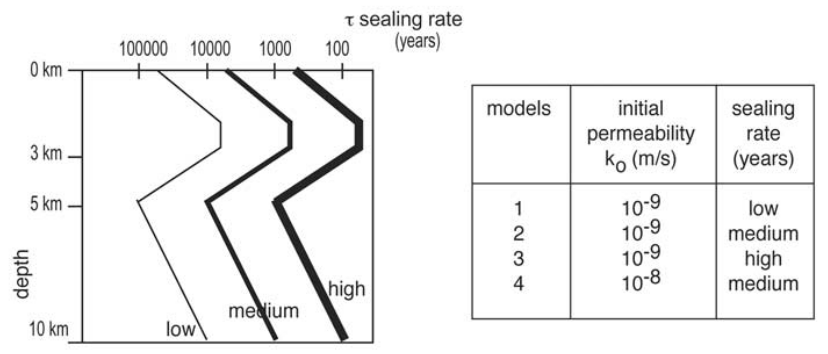
\includegraphics[width=15cm]{python_codes/fieldstone_126/images/grfr03a}\\
{\captionfont 
Left (Fig. 9a): Synthetic variation
in crack sealing rate with depth integrating two superimposed calcite-rich and quartz-rich levels: crack
sealing is modeled with pure calcite between 0 and 3 km, pure quartz between 5 and 10 km and
intermediate behavior between 3 and 5 km. Crack sealing is expressed as the t values (time require in
order to divide the initial porosity by 2.72). Three sets of crack sealing values are derived from this
section: low, medium and high sealing rate profiles.
Right (Fig. 9b): Table of values of the main modeling parameters:
initial permeability $k_0$ and sealing rate. 
The initial porosity along the fault is 10\% (Figures 9c, 10, and 11) or 1\% (Figures 12 and 13).}
\end{center}


\begin{center}
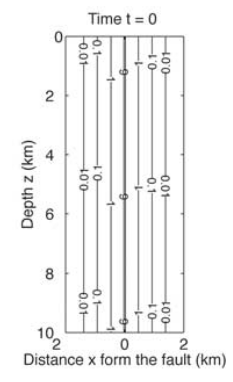
\includegraphics[width=7cm]{python_codes/fieldstone_126/images/grfr03b}\\
{\captionfont Fig. 9c: initial porosity profile.}
\end{center}


%%%%%%%%%%%%%%%%%%%%%%%%%%%%%%%%%%%%%%%%%%%%%%%%%%%%%%%%%%%%%%%%
\newpage
\section*{FEM discretisation and code structure}

Based on Fig 9, the domain is a Cartesian box of size $4~\si{\km} \times 10~\si{\km}$ (also from paragraph 45). In the paper the vertical $z$ axis points down (note that our code will obviously 
not follow this convention and that the axis will be $x,y$ as usual). 
Note that the domain is in fact $[-2:2]\times[0:10]~\si{\km}$. 
From Eq.~\eqref{eq:por02} and various figures we know that we are solving for the overpressure $p$. 
\[
C \upphi_m \frac{\partial p}{\partial t} 
=\frac{\partial}{\partial x} \left( K_x \frac{\partial p}{\partial x} \right) 
+ \frac{\partial}{\partial z} \left( K_z \frac{\partial p}{\partial z} \right)
- \frac{\partial \upphi_m}{\partial t} 
%=\frac{\partial}{\partial x} \left( K_x \frac{\partial p}{\partial x} \right) 
%+ \frac{\partial}{\partial z} \left( K_z \frac{\partial p}{\partial z} \right)
%+\frac{\upphi_0}{\tau(z)} \exp (-x/L) \exp (-t/\tau(z)) 
\]
which is a diffusion equation in 2d, with a source term. 
This equation must be supplemented by equations for $K_x(x,z,t)$, $K_z(x,z,t)$, $\upphi_m(x,z,t)$ and 
$\frac{\partial \upphi_m}{\partial t} (x,y,t)$, i.e. Eqs.~\eqref{eq:por06}, \eqref{eq:por07}, \eqref{eq:por03}, \eqref{eq:por04}:
\begin{eqnarray}
K_x(x,z,t) &=& \frac{k_0 }{\rho_m g}  \exp\left(-\frac{x}{L}\right) \exp\left(-3\frac{t}{\tau(z)}\right) \nn\\
K_z(x,z,t) &=& 100\frac{k_0 }{\rho_m g}  \exp\left(-\frac{x}{L}\right) \exp\left(-3\frac{t}{\tau(z)}\right) \nn\\
\upphi_m(x,z,t) &=& \upphi_0 \exp (-x/L) \exp (-t/\tau(z)) \nn\\
\frac{\partial \upphi_m}{\partial t}(x,z,t) &=& -\frac{\upphi_0}{\tau(z)} \exp (-x/L) \exp (-t/\tau(z)) \nn
\end{eqnarray}
Finally we will need the parameters $k_0$, $\rho_m$, $g$, $\upphi_0$, $L$, $C$ and the curve $\tau(z)$.
They have all been specified in the text above:

\begin{itemize}
\item $k_0 = 10^{-9}~\si{\meter\per\second}$ or $10^{-8}~\si{\meter\per\second}$
\item $\rho_m=880~\si{\kg\per\cubic\meter}$, 
\item $g=10~\si{\meter\per\square\second}$, 
\item $\rho_{litho}=2800~\si{\kg\per\cubic\meter}$, 
\item $L=100~\si{\meter}$, 
\item $C=10^{-9}~\si{\per\pascal}$.
\item $\phi_0=1\%,10\%$ is a maximum porosity value along the fault, the initial porosity profile shows an
exponential decrease away from the fault
\end{itemize}

Note that there is a discussion about pressure in Eq.\eqref{eq:por08} that needs to be implemented.

%..........................................
\paragraph{Some thoughts about $\tau(z)$}

I have digitized\footnote{\url{https://plotdigitizer.com/app}} Fig.~9a:
\begin{center}
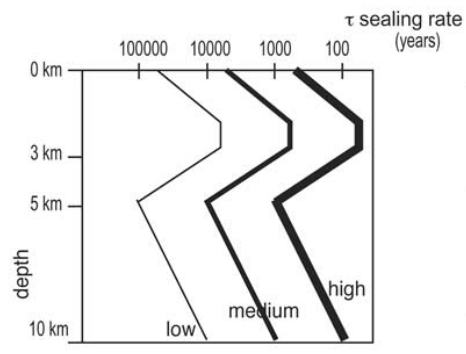
\includegraphics[width=8cm]{python_codes/fieldstone_126/images/grfr03f}
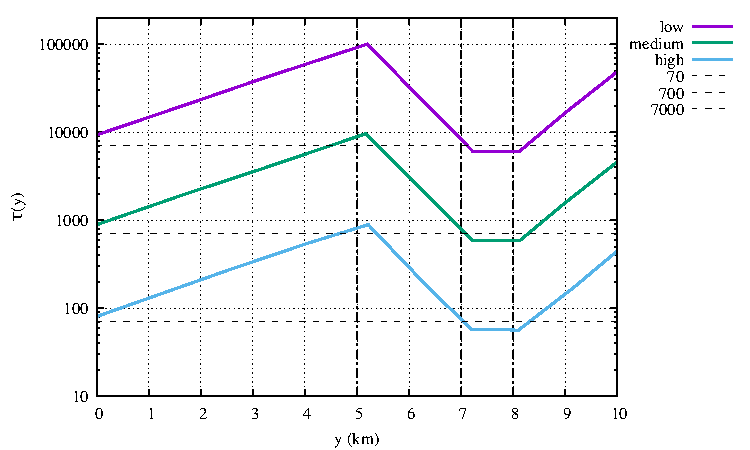
\includegraphics[width=8cm]{python_codes/fieldstone_126/images/tau.pdf}\\
{\captionfont Left: Fig.~9a of the paper; Right: digitized version, note that $y$ is not depth but the
vertical coordinate.}
\end{center}
The original figure is obviously poorly put together and serves as an indication rather than 
an accurate representation of the sealing rate $\tau$.
The three broken lines are identical but off by a factor 10.  
Fig.~10 showcases the parameter $\tau_m=70yr,700,7000yr$ which is not discussed in the text (CHECK)
but which seems to correspond to the flat portions of the curves of Fig.~9a.

In the paper we read ``
In the upper crust, we assume the predominance of the calcite rate of crack sealing
at low temperature and pressure while in the deeper crust we
assume the predominance of the rate of crack sealing of the
quartzite at higher temperature and pressure [Renard et al.,2000]. 
The depth of transition between these two end-member cases is chosen to be at 3 km.''
Looking at the digitized figure it is obvious the figure is incorrect. The 3km-depth 
line (i.e. the $y=7~\si{\km}$ line) does not align with the transition of the curves.
Also it appears that  the flat sections are nowhere discussed in the text (CHECK).

In light of all this we will write a single function that returns $\tau$ as a function of $y$
and it will correct the problems highlighted above. 
For the `low' curve: it starts at (0,10000), goes to (5,100000), then to (7,7000), plateaus
until (8,7000) and then goes up to (10,:50000).
The other two lines follow the same pattern but their $\tau$ values are a factor 10 and 100 lower.
The function is then as follows:
\begin{lstlisting}
def tau_fct(y,srcoeff):
    if y<5.e3:
       val=1e4+y/5e3*(1e5-1e4)
    elif y<7e3:
       val=1e5-(y-5e3)/(7e3-5e3)*(1e5-7000)
    elif y<8e3:
       val=7000
    else:
       val=7000+(y-8000)/(10e3-8e3)*(50000-7000)
    return val*year*srcoeff
\end{lstlisting}
The \lstinline{srcoeff} is either 1 (hight sealing rate), 0.1 (medium sealing rate)
or 0.01 (high sealing rate).


%..............................
\paragraph{Initial conditions}

%paragraph 45
Just after an earthquake, the initial condition at $t=0$ is $p=0$ (and consequently 
$\upphi'=0$  and $\rho'=0$).

%..............................
\paragraph{Boundary conditions}

%paragraph 45
The calculation was based on the following boundary conditions: 
\begin{itemize}
\item top: $p=0$;
\item sides:  hydrostatic pressure, i.e., $p=0$;
\item bottom: imposed pressure zone scaled
with the fault zone, i.e., $p = g h (\rho_{litho} -\rho_m) e^{-x/L}$ which is plotted here under: 
\begin{center}
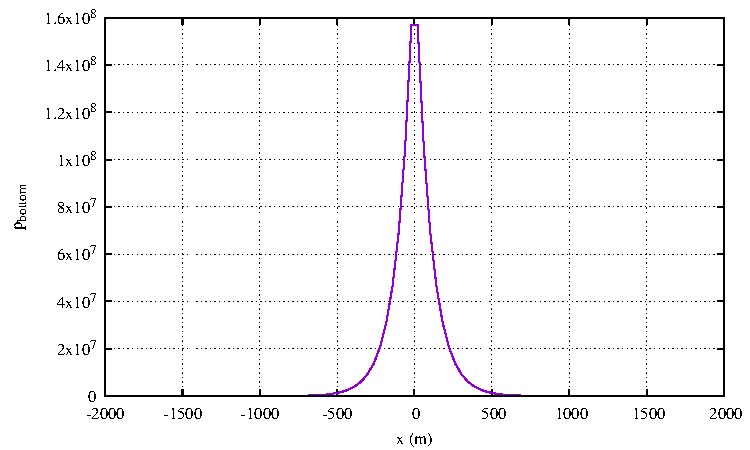
\includegraphics[width=7cm]{python_codes/fieldstone_126/images/pbottom}\\
{\captionfont Pressure imposed at the bottom.}
\end{center}
The maximum value is then $g h (\rho_{litho} -\rho_m) =10*40e3*(2800-880)=192~\si{\mega\pascal}$.

\end{itemize}
I suspect the authors to only solve for half the domain (bc of symmetry) since they 
specify boundary conditions on the fault. Also the expressions for $K$ contain $\exp(-x/L)$
instead of $\exp(-|x|/L)$.



%..............................
\paragraph{Weak form}

How to establish the weak form of the diffusion equation has been 
carried out in Section~\ref{MMM-ss:hte_fem} so we will not repeat it. 
The only main difference from the standard diffusion equation for temperature
is the coefficients and the source term which are all space and time dependent.

The discretised weak form is given by
\[
\underbrace{
\left( \int_\Omega \vec{\bN}^T \upphi_m C  \vec{\bN} dV  \right)
}_{\M}
 \cdot \frac{\partial \vec{\cal P}}{\partial t}
+
\underbrace{
\left( \int_\Omega {\bm B}^T \cdot  {\bm K} \cdot {\bm B} dV \right)
}_{{\K}_d}
 \cdot \vec{\cal P}
=
\underbrace{
-
\int_\Omega \vec{\bN}^T  \frac{\partial \upphi_m}{\partial t} dV
}_{\vec{b}}
\]
Since pressure is prescribed on all sides the surface terms stemming from the integration by parts
need not be taken into account here.

The time derivative can be discretised by means of a simple explicit scheme:
\[
\frac{\partial \vec{\cal P}}{\partial t} \simeq
\frac{ \vec{\cal P}^{t+\delta t} - \vec{\cal P}^t  }{\delta t}
\]
We arrive at 
\[
( {\M} + {\K}_d) \cdot \vec{\cal P}^{t+\delta t} = {\M} \cdot \vec{\cal P}^t  + \vec{b}
\]
The matrix is symmetric positive definite which is good news.


%..............................
\paragraph{Logic of the code}

\begin{enumerate}
\item define all required parameters
\item set $p=0$ everywhere
\item set profile for $\tau(z)$
\item define boundary conditions
\item define mesh, connectivity array
\item etc ...
\end{enumerate}

%..............................
\paragraph{Numerical experiments:} From Fig.~9b we see that four models are run:
\begin{itemize}
\item model 1: $k_0=10^{-9}~\si{\meter\per\second}$, low sealing rate
\item model 2: $k_0=10^{-9}~\si{\meter\per\second}$, medium sealing rate
\item model 3: $k_0=10^{-9}~\si{\meter\per\second}$, high sealing rate
\item model 4: $k_0=10^{-8}~\si{\meter\per\second}$, medium sealing rate
\end{itemize}



\newpage

%======================================
\section*{Results}

\begin{center}
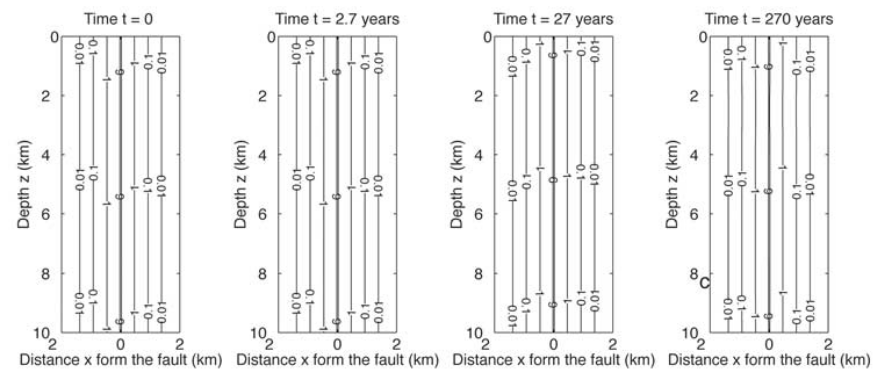
\includegraphics[width=14cm]{python_codes/fieldstone_126/images/grfr03c}\\
{\captionfont Fig. 9c: Evolution of the porosity values with time (t), through crustal cross
section perpendicular to the fault (located at x = 0); 
evolution is obtained with the lowest sealing rate (model 1, Figure 9b),
initial porosity profile}
\end{center}

\begin{center}
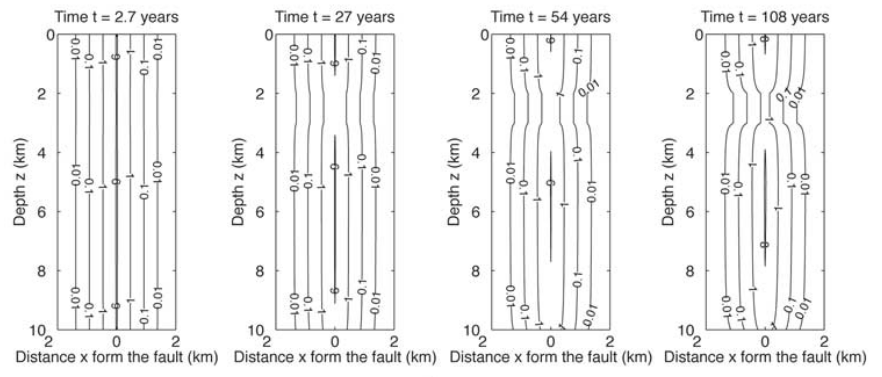
\includegraphics[width=14cm]{python_codes/fieldstone_126/images/grfr03d}\\
{\captionfont Fig. 9d: same as Fig. 9c, but evolution is 
obtained with the highest sealing rate (model 3, Figure 9b).}
\end{center}


\newpage

Fluid transfer modeling along active crustal faults when integrating pressure solution crack sealing
processes in parallel with inflow of deep lower crust fluids (see Figure 9b); evolution of 
normalized fluid overpressure $O_{vp} = p/(P_{litho}-P_{hydro}) = (P- P_{hydro})/(P_{litho} - P_{hydro})$. 
This quantity is between 0 and 1 and it is the quantity plotted on the following plots:
\begin{center}
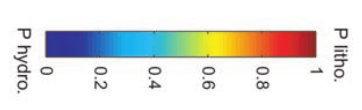
\includegraphics[width=6cm]{python_codes/fieldstone_126/images/grfr03_Ovp}\\
\end{center}
The initial porosity along the fault surface is 10\%. Time-dependent
variation is from left to right (from 2.7 to 270 years). The $\tau$ values are the time duration 
requires in order to divide the initial porosity by $e$ (see Figure 9a). 

\begin{center}
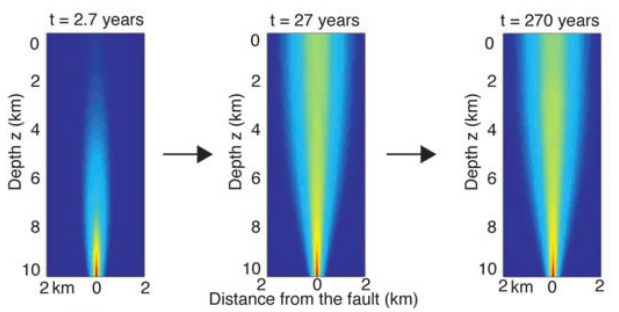
\includegraphics[width=13cm]{python_codes/fieldstone_126/images/grfr03_10a}\\
{\captionfont Fig. 10a:
(a) Model 1, initial permeability $k_0 = 10^{-9} m/s$, low sealing rate; 
overpressure rapidly increases at depth (zone with $O_{vp}$ values = 0.9) then very 
slowly extends to the entire fault zone ($O_{vp}$ values reaching 0.6
after several hundred years). 
}
\end{center}

\begin{center}
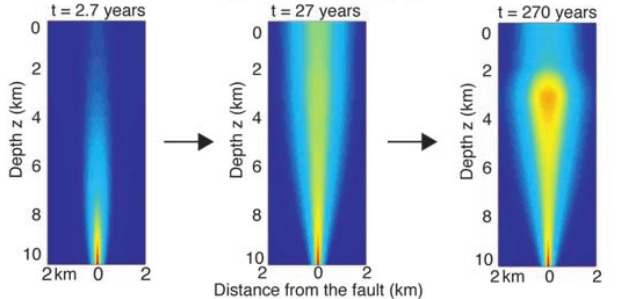
\includegraphics[width=13cm]{python_codes/fieldstone_126/images/grfr03_10b}\\
{\captionfont Fig. 10a:
Model 2, initial permeability $k_0 = 10^{-9} m/s$, medium sealing rate; same fast localized
overpressure development at depth (red zone) slowly extending to the whole fault. However, 
medium sealing rate allows localized overpressure development in the upper part 
of the seismic crust (270 years). 
}
\end{center}

\begin{center}
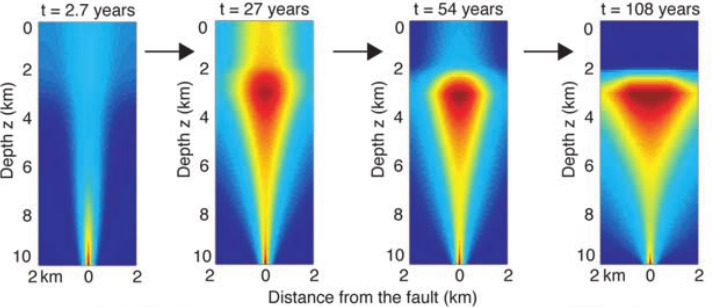
\includegraphics[width=13cm]{python_codes/fieldstone_126/images/grfr03_10c}\\
{\captionfont Fig. 10c:
Model 3, initial permeability $k0 =10^{-9} m/s$, high sealing rate; same fast localized overpressure 
development at depth (red zone). However, high sealing rate rapidly develops localized overpressure 
in the upper part of the seismic crust and prevents the outflow of the fluid (before 108 years). 
}
\end{center}

\begin{center}
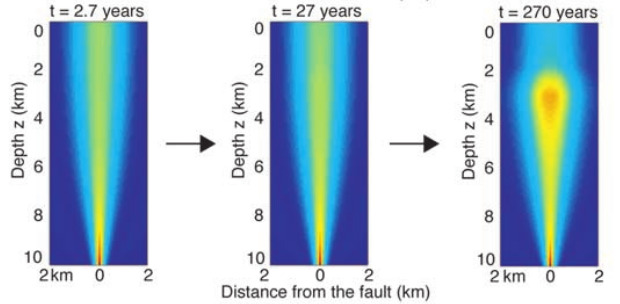
\includegraphics[width=13cm]{python_codes/fieldstone_126/images/grfr03_10d}\\
{\captionfont Fig. 10d:
Model 4, initial permeability $k_0 = 10^{-8} m/s$, 
medium sealing rate; same fast localized overpressure
development at depth (red zone) rapidly extending to the whole fault after some years 
($e$ years), contrary to model 2. However, even with the effect of medium sealing rate values, 
localized overpressure finally develops in the upper part of the seismic crust as in model 2 (270 years).
}
\end{center}




